\section{Bäume}
%Kommentar
\begin{definition}
Ein Graph $G$ heißt \emph{azyklisch} oder \emph{zyklenfrei}, falls es keine Zyklen in $G$ gibt. Ein ungerichteter, azyklischer und zusammenhängender Graph ist ein \emph{Baum}
\end{definition}
\begin{example}
Ein azyklischer Graph kann wie folgt aussehen:
\begin{center}
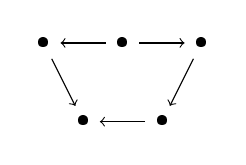
\begin{tikzpicture}
	\node (1) at (0,0) {•};
	\node (2) at (1,0) {•};
	\node (3) at (-1,0) {•};
	\node (4) at (0.5,-1) {•};
	\node (5) at (-0.5, -1) {•};


	\path [->] (1) edge node {} (2);
	\path [->] (1) edge node {} (3);
	\path [->] (2) edge node {} (4);
	\path [->] (4) edge node {} (5);
	\path [->] (3) edge node {} (5);	
\end{tikzpicture}
\end{center}
Sollte dieser ungerichtet sein könnte er so aussehen:
\begin{center}
\begin{tikzpicture}
	\node (1) at (0,0) {•};
	\node (2) at (2,0) {•};
	\node (3) at (1,-1) {•};
	\node (4) at (3,-1) {•};
	
	\node (5) at (-2,0) {•};
	\node (6) at (-1,-1) {•};
	\node (7) at (-3,-1) {•};

	\path [-] (1) edge node {} (2);
	\path [-] (1) edge node {} (5);
	\path [-] (2) edge node {} (3);
	\path [-] (3) edge node {} (4);
	\path [-] (5) edge node {} (6);
	\path [-] (5) edge node {} (7);
\end{tikzpicture}
\end{center}
Dieser Graph ist sogar zusammenhängend.
\end{example}
\begin{theorem}
Sei $G=(V,E)$ ein ungerichteter Graph mit $n=|V|$ knoten. Dann sind die folgenden Aussagen äquivalent.
\begin{enumerate}
	\item G ist ein Baum
	\item G hat n-1 Kanten und ist zusammenhängend
	\item G hat n-1 Kanten und ist azyklisch
	\item G ist azyklisch und das Hinzufügen einer beliebigen, noch nicht vorhandenen Kante erzeugt einen Zyklus.
	\item G ist zusammenhängend und das Entfernen einer beliebigen Kante macht G unzusammenhängend.
	\item Jedes Paar verschiedener Knoten in G ist durch genau einen einfachen Weg miteinander verbunden.
\end{enumerate}
\end{theorem}
\begin{proof}
Wir zeigen nicht jede Äquivalenz einzeln, sondern folgern aus anderen Aussagen.\begin{itemize}
	\item \underline{$a \implies f$} Falls es für ein gegebenes Paar $v,w \in  V$, verschiedene Wege gäbe, so würde die Vereinigung dieser beiden Wege einen Zyklus beinhalten (Widerspruch zu azyklisch in Baum).
	\item \underline{$f \implies e$} "zusammenhängend" folgt per Definition.
		Falls wir eine beliebige Kante entfernen, so sind die beiden Endpunkte nicht mehr voneinander erreichbar ( $\implies$ G wird unzusammenhängend).
	\item \underline{$e \implies d$} G ist azyklisch, da wir sonst eine (ausgewählte) Kante entfernen könnten, so dass g immer noch zusammenhängend wäre. Seien $v,w \in  V, w \neq v$, dann gibt es einen Weg von v nach w. 
	Hinzufügen der Kante $\{v,w\}$ macht diesen Weg zum Zyklus.
\item \underline{$d \implies c$} Wir zeigen per Induktion über $m= |E|$, dass für einen azyklischen, ungerichteten Graph
	\begin{equation}
	\label{eqn:keinplan}
		n=m+p
	\end{equation}
	gilt, wobei p die Anzahl Zusammenhangskomponenten ist.
	\begin{itemize}[label=$\lozenge$, itemsep=2ex]
		\item IV \underline{$m=0$} trivial
		\item IS \underline{$m \to m+1$} Beim Hinzufügen einer Kante muss eine Zusammenhangskomponente verschwinden, da sonst ein Zyklus entstehen würde. \\
	Da das Hinzufügen einer beliebigen neuen Kante einen Zyklus entstehen lässt, muss $p=1$ gelten.
	\[
	\implies |E|=m=n-1
	\]
	\end{itemize}
\item \underline{$c \implies b$} Folgt aus \eqref{eqn:keinplan}
\item \underline{$b \implies a$} Zu zeigen: $G$ ist azyklisch. \\
	Angenommen $G$ hat $k$ verschiedene einfache Zyklen. Dann können wir $G$ durch entfernen von $k$ Kanten zu einem azyklischen Graphen machen. \eqref{eqn:keinplan} ist andwendbar, un impliziert, dass 
	\begin{align*}
		n &= (m-k)+1 \\
		m+1 &= (m-k)+1 		    &\implies k=0
	\end{align*}
	d.h. $G$ keine Zyklen.
\end{itemize}
\end{proof}
\begin{remark}
Fixieren wir in einem Baum $G=(V,E)$ einen Wurzelknoten, so wird automatisch eine Richtung in den Kanten festgelegt. Für $v \in V$ heißt $pre(v), |pre(v)|=1$ der \emph{Elternteil} und $post(v)$ die \emph{Kinder}.
\end{remark}
